\documentclass[tikz,border=1pt]{standalone}
\usetikzlibrary{calc,decorations.pathmorphing,patterns,positioning,shapes,shadings}

\usepackage{bm}
\usepackage{amsmath}

\definecolor{purple}{RGB}{147,7,204}
\definecolor{green}{RGB}{5,100,18}
\definecolor{blue}{RGB}{10,153,201}
\definecolor{red}{RGB}{213,42,45}
\definecolor{orange}{RGB}{254,128,41}
\definecolor{gray}{RGB}{239,240,241}

\pgfdeclarelayer{bg}
\pgfsetlayers{bg,main}

\renewcommand{\vec}[1]{\bm{#1}}
\newcommand{\mat}[1]{\bm{#1}}

\begin{document}
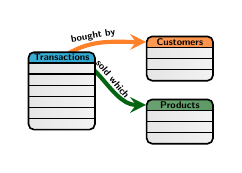
\begin{tikzpicture}

\def\boxwidth{15pt}
\def\boxheight{15pt}

\tikzset{line/.style={draw,semithick}}
\tikzset{arrow/.style={line,->,>=stealth}}
\tikzset{textnode/.style={inner sep=0pt}}
\tikzset{node/.style={circle,inner sep=0pt,minimum width=15pt}}
\tikzset{box/.style={line,inner sep=0pt,minimum width=\boxwidth,minimum height=\boxheight}}
\tikzset{snake/.style={arrow,very thick,decorate,decoration={snake,amplitude=1,segment length=6,post length=5}}}
\tikzset{gradient/.style={shading=axis,shading angle=-45}}
\tikzset{legend/.style={node,rectangle,minimum width=8pt,minimum height=8pt,rounded corners=2pt,draw=none}}

\tikzset{orangenode/.style={line,node,gradient,left color=orange!80!white,right color=orange!85!white}}
\tikzset{bluenode/.style={line,node,gradient,left color=blue!80!white,right color=blue!85!white}}
\tikzset{graynode/.style={line,node,gradient,left color=white!90!black,right color=white!95!black}}



\tikzset{pics/history/.style args={#1}{code={%
  % \node (#1) at (0,0) {};

  % \node[line,rectangle,minimum width=24pt,minimum height=28pt] at (0, 0) {};

  \node[rectangle,minimum width=24pt,minimum height=4pt,inner sep=0pt,gradient,left color=blue!80!white,right color=blue!85!white] at (0,12pt) (#1) {};
  \node[rectangle,minimum width=24pt,minimum height=24pt,inner sep=0pt,left color=white!90!black,right color=white!95!black] at (0,-2pt) {};

  \path[line] (-12pt,10pt) to (12pt,10pt);
  \path[line] (-12pt,6pt) to (12pt,6pt);
  \path[line] (-12pt,2pt) to (12pt,2pt);
  \path[line] (-12pt,-2pt) to (12pt,-2pt);
  \path[line] (-12pt,-6pt) to (12pt,-6pt);
  \path[line] (-12pt,-10pt) to (12pt,-10pt);

  \draw[white,fill=white] (-12pt,14pt) -- (-11pt,14pt) -- (-12pt,13pt) -- cycle;
  \draw[white,fill=white] (12pt,14pt) -- (11pt,14pt) -- (12pt,13pt) -- cycle;

  \draw[white,fill=white] (-12pt,-14pt) -- (-11pt,-14pt) -- (-12pt,-13pt) -- cycle;
  \draw[white,fill=white] (12pt,-14pt) -- (11pt,-14pt) -- (12pt,-13pt) -- cycle;
  \node[line,rectangle,minimum width=24pt,minimum height=28pt,rounded corners=2pt] at (0,0) {};
}}}

\tikzset{pics/historysmall/.style args={#1}{code={%
  % \node (#1) at (0,0) {};

  % \node[line,rectangle,minimum width=24pt,minimum height=28pt] at (0, 0) {};

  \node[rectangle,minimum width=24pt,minimum height=4pt,inner sep=0pt,gradient,left color=orange!80!white,right color=orange!85!white] at (0,12pt) (#1) {};
  \node[rectangle,minimum width=24pt,minimum height=12pt,inner sep=0pt,left color=white!90!black,right color=white!95!black] at (0,4pt) {};

  \path[line] (-12pt,10pt) to (12pt,10pt);
  \path[line] (-12pt,6pt) to (12pt,6pt);
  \path[line] (-12pt,2pt) to (12pt,2pt);

  \draw[white,fill=white] (-12pt,14pt) -- (-11pt,14pt) -- (-12pt,13pt) -- cycle;
  \draw[white,fill=white] (12pt,14pt) -- (11pt,14pt) -- (12pt,13pt) -- cycle;

  \draw[white,fill=white] (-12pt,-2pt) -- (-11pt,-2pt) -- (-12pt,-0pt) -- cycle;
  \draw[white,fill=white] (12pt,-2pt) -- (11pt,-2pt) -- (12pt,-0pt) -- cycle;
  \node[line,rectangle,minimum width=24pt,minimum height=16pt,rounded corners=2pt] at (0,6pt) {};
}}}

\tikzset{pics/historytrain/.style args={#1}{code={%
  % \node (#1) at (0,0) {};

  % \node[line,rectangle,minimum width=24pt,minimum height=28pt] at (0, 0) {};

  \node[rectangle,minimum width=24pt,minimum height=4pt,inner sep=0pt,gradient,left color=green!60!white,right color=green!65!white] at (0,12pt) (#1) {};
  \node[rectangle,minimum width=24pt,minimum height=12,inner sep=0pt,left color=white!90!black,right color=white!95!black] at (0,4pt) {};

  \path[line] (-12pt,10pt) to (12pt,10pt);
  \path[line] (-12pt,6pt) to (12pt,6pt);
  \path[line] (-12pt,2pt) to (12pt,2pt);

  \draw[white,fill=white] (-12pt,14pt) -- (-11pt,14pt) -- (-12pt,13pt) -- cycle;
  \draw[white,fill=white] (12pt,14pt) -- (11pt,14pt) -- (12pt,13pt) -- cycle;

  \draw[white,fill=white] (-12pt,-2pt) -- (-11pt,-2pt) -- (-12pt,-0pt) -- cycle;
  \draw[white,fill=white] (12pt,-2pt) -- (11pt,-2pt) -- (12pt,-0pt) -- cycle;
  \node[line,rectangle,minimum width=24pt,minimum height=16pt,rounded corners=2pt] at (0,6pt) {};
}}}


\pic at (0, 0) {history=history1};
\pic at (1.5,0.2) {historysmall=history2};
\pic at (1.5,-0.6) {historytrain=history3};

\node[textnode, scale=0.35] at (1.5,-0.18) {\sffamily \textbf{Products}};
\node[textnode, scale=0.35] at (1.5,0.62) {\sffamily \textbf{Customers}};
\node[textnode, scale=0.35] at (0,0.425) {\sffamily \textbf{Transactions}};

\node[textnode, scale=0.35, rotate=310] at (0.65,0.15) {\sffamily \textbf{sold which}};
\node[textnode, scale=0.35, rotate=10] at (0.4,0.7) {\sffamily \textbf{bought by}};
\begin{pgfonlayer}{bg}

%\node[textnode] at (10.0,0.8) {\small CPU};

\path[arrow,color=orange,line width=1.5pt,in=180,out=35] (history1.center) to (history2.west){};
\path[arrow,color=green,line width=1.5pt,in=180,out=35] (history1.south) to (history3.west);

\end{pgfonlayer}

\end{tikzpicture}
\end{document}